\documentclass[main.tex]{subfiles}
\begin{document}
	\chapter{Introduction}
	\chapterauthor{Merete Bommarius, Torge Olliges}
	\label{introduction}
	
	This is the documentation for the SUTURO project of 2019/2020. The goal was the successful participation in the RoboCup@Home with the Human Service Robot. \\
	The Human Service Robot also referred to as HSR is a robot designed by Toyota. Its purpose is to help humans in their daily life and perform simple tasks like cleaning, tidying up et cetera. The RoboCup is a yearly tournament dedicated to robots that have to accomplish specific tasks. Participants come from all over the world and are required to bring their own robot.
During the RoboCup, the HSR had to perform different tasks autonomously.
This year the group chose to focus on the tasks “Storing Groceries“ and “Clean Up“, as found in the Rulebook of 2019, which can be found on the \href{http://www.robocupathome.org/rules}{RoboCup@Home website}. 
	Storing Grocery entails that the HSR has to store groceries into a pantry shelf, sorting them into appropriate groups determined by the items that are already placed on all shelf floors. The items that the HSR has to store are located on a table in the same room as the pantry shelf.
Clean Up is a different task for which the HSR has to tidy up a room with assorted objects. The objects, have to be brought to their determined locations. Unidentified objects have to be placed in the garbage bin. In comparison to Storing Groceries, the objects from Clean Up can be located anywhere in the arena. This includes the floor, seats, and other furniture.
Due to specific circumstances, which will be explained later in the documentation, the group was not able to work on the HSR itself during the third and final milestone and switched to a virtual substitute.
	In the following sections, the challenges that were encountered will be described, each subgroup of the project will elaborate on their work, and in the end, there will be a section of ideas on how to improve the project for the next generation of SUTURO.
	
	\section{Challenges}
	\label{challanges}
	\chapterauthor{Torge Olliges, Marc Stelter,\\ Jeremias Thun}
	Working with the robot, the human intuition about what should be done, what can be recognized, how should everything be ordered needs to be translated into a specific way to work with camera data, to automatically organize the data or to have stable movements that can always be repeated that way.\\
	
	\begin{figure}[H]
		\centering
		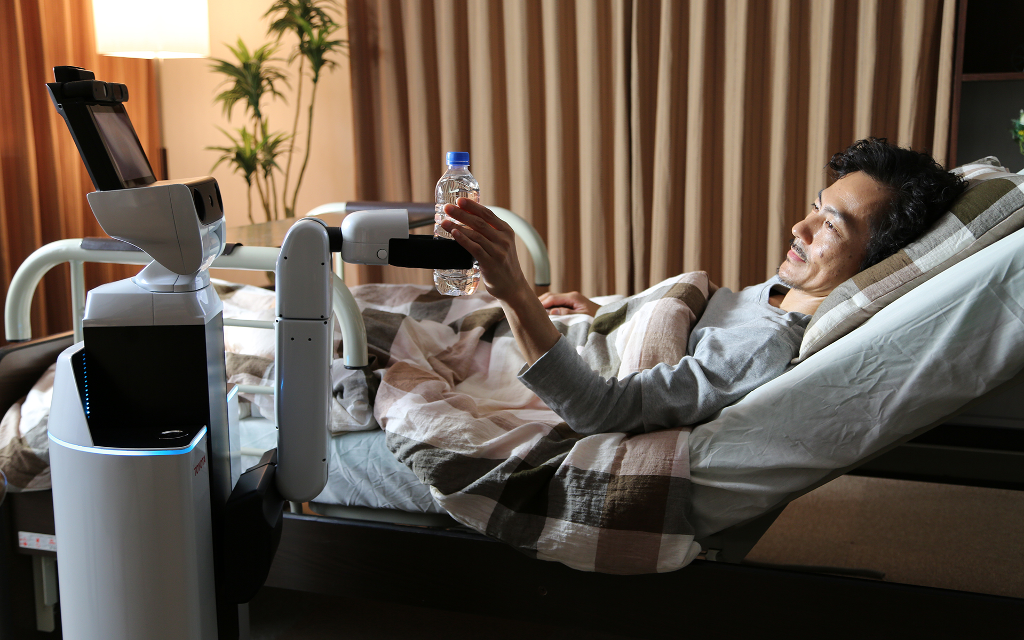
\includegraphics[scale=0.375]{pictures/front_page_hsr}
		\caption{Source: \href{www.hsr.io}{hsr.io}}
	\end{figure}
	
	For this SUTURO group, this resulted in several challenges which had to be faced:
	\begin{itemize}
		\item Navigation: To get from one position to another, e.g. to a table, shelf or object. The robot has to be able to perform these navigation actions autonomously.
		\item Localization: The robot needs to know where it is located. The robot has to handle the problem that the pose estimation is not perfect in a real-life scenario.
		\item Detection: The robot has to be able to find objects without prior knowledge of their position.
		\item Recognition: The robot has to be able to recognize objects, work with bad lighting conditions, and noise in images.
		\item Classification: The robot has to be able to classify objects depending on their size, color, shape and type. The robot has to be able to handle unknown objects.
		\item Sorting: When placing the objects, the robot has to sort them in a way, that humans can intuitively agree on.
		\item Manipulation: The robot has to be able to interact with its environment grasping and placing objects while avoiding collisions.
		\item Manipulation: The robot needs to take different poses to move or look at an object.
		\item Communication: To communicate what the robot does and which decisions it makes, it needs to be able to have voice output.
		\item Running stable: The robot has to be able to adapt to changes in its environment.
		\item Decision making: Decisions have to be made according to the current environment, they can not be predefined. 
		\item Timing: During the RoboCup each task has a limited time frame.
	\end{itemize}

	\section{Previous Work}
    \label{previous_work}
    \chapterauthor{Torge Olliges, Paul Schnipper, \\Jan Neumann, Jan-Frederik Stock}
		The SUTURO project is a reoccurring project hosted by the iai-office at the University of Bremen. Therefore, the current project could rely on previous work and insights in the form of legacy code and experience. Especially about the difficult conditions during the RoboCup and the challenges working with the HSR. In this section a brief overview of the legacy code will be given by every group:
	\subsection{Planning}
		Although most of the code was changed and tweaked to fit the new requirements the general structure of the previous group was used. Some of the Interfaces were reused for example the interface for the navigation client and the interface to \textit{RoboSherlock} (\ref{object-perceive}). Some of the mid-level functionality like the designators (\ref{desig}) and process module code (\ref{pcm}) were reused and altered to fit the new means.
	\subsection{Navigation}
		The HSR already comes with its own navigation setup. This includes a static and dynamic obstacle map, in addition to a path planner. During previous runs of the project snap\_map\_icp has been introduced improving localization. The static map is created with hector\_slam.
	\subsection{Manipulation}
		Even though there was an existing legacy code for Manipulation, the decision was made to abandon that code and start from scratch. This was recommended by the tutors because the \textit{Giskard} framework had evolved significantly since then. As a result Manipulation only used the \textit{Giskard} framework and no legacy code.
	\subsection{Perception}
	The perception group used two packages of previous SUTURO generations, namely the rs\_hsrb\_perception package and the rs\_turn\_table package.
	
	 The rs\_hsrb\_perception package contains a process manager for \textit{RoboSherlock} and modified annotators, to annotate regions. It was used by the perception group to be able to load multiple pipelines simultaneously and it was adapted to work with the newest \textit{RoboSherlock} version.
	 
	 The rs\_turn\_table package is a package which is used to record image data for classification. This was used by the perception group without any changes. 
	\subsection{Knowledge}
        The previous codebase was designed around the storing groceries task. Because this year's team decided to also try the Clean-Up task, the knowledge base had to be adapted. Even though every \textit{Prolog} predicate got changed, the code deciding the goal position of the object and the methodology of using ontologies to find similar objects, are still kept.
    \subsection{NLP}
        Previously no speech-to-text capabilities where part of the codebase. Sentences were and still are hardcoded in the planning and knowledge modules.
\end{document}



